\subsection{premi/client/presentationManager}
%diagramma del package%
\begin{figure}[h]
\begin{center}
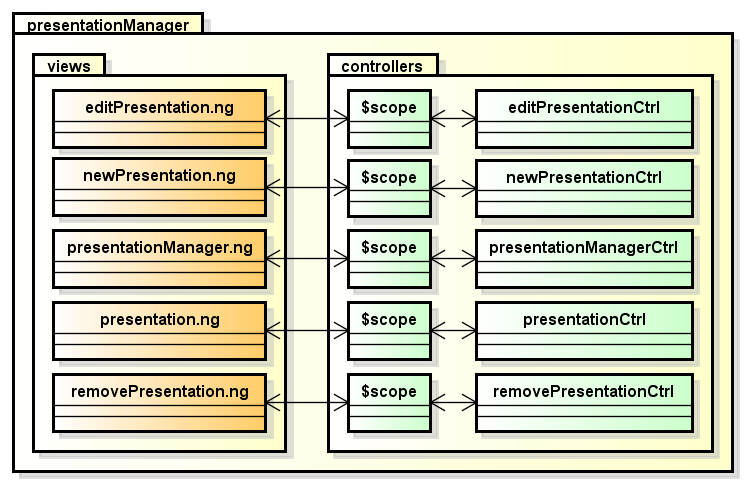
\includegraphics[scale=0.50]{img/diapkg/presentationManager.png}
\caption{Diagramma del package premi/client/presentationManager}
\end{center}
\end{figure}


%-------  diagramma della classe%
\subsubsection{premi/client/}
\begin{figure}[h]
\begin{center}
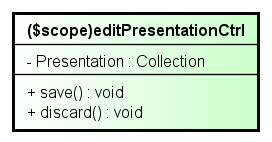
\includegraphics[scale=0.90]{img/diacla/editPresentationCtrl.png}
\caption{Diagramma della classe premi/client/presentationManager/editPresentationCtrl}
\end{center}
\end{figure}




\begin{description}
%-------  descrizione della classe%
\item[Descrizione] \hfill \\
	Controller della view \textit{editPresentation.ng}
	

%-------  lista delle classi associate%	
\item[Associazioni] \hfill \\
	\begin{itemize}
		\item \textbf{classe/associata}: per fare cosa?
	\end{itemize}

	
%-------  lista degli Attributi%	
\item[Attributi] \hfill \\
	\begin{description}
		\item[\textbf{- int attributo1			}] \hfill \\
			Descrizione dell'attributo
		\item[\textbf{- int attributo2			}] \hfill \\
			Descrizione dell'attributo
	\end{description}
	
	
%-------  lista dei metodi%	
\item[Metodi] \hfill \\

	% -- inizio metodo -- %
	\begin{description}
		\item[\textbf{\color{blue}+ void operation0()			}] \hfill \\
			Descrizione del metodo
			
		\begin{description}
			% -- lista argomenti del metodo -- %
			\item[Argomenti] \hfill \\
				\begin{itemize}
				
					\item \textbf{nomeArgomento : tipoArgomento			} \hfill \\
					Descrizione argomento
					
				\end{itemize}
			% -- note aggiuntive sul metodo -- %
			\item[Note] \hfill \\
			\begin{itemize}
					\item Deve essere esplicitamente marcato come costante (?)
					\item Deve possedere qualche caratteristica
					\item Metodo ridefinito
				\end{itemize}
		\end{description}
	\end{description}
	% -- fine metodo -- %		
	
	
	
\end{description}
